\section{Charactersitics of real-time transit data}
\label{sec:realtime-data}

There are a range of \gls{avl} technologies which allow transit vehicles to report their locations in real-time. The most common of these is now the \gls{gps}, which provides the longitude and latitude of the vehicle. In the simplest of deployments, each vehicle reports its location to a central server at a fixed time interval. The server then collates the reports from all buses in the fleet and makes them available via an \gls{api}.


Another type of real-time data available to us is arrival and departure information at bus stops. When a vehicle arrives at or departs from a stop,\footnote{Or thinks it does, see \cref{sec:vp_data}.} it reports to the server which stop it is at, and its time of arrival or departure. The server then computes the delay (the time between actual and scheduled arrival or departure), collates the data from multiple vehicles, and also makes these available through an \gls{api}.


Real-time vehicle information can be displayed in one of two ways. \Gls{gps} positions are displayed on a map accessed through a mobile app, allowing commuters to see where their bus was when it last reported its location. For trip updates, the \emph{current delay} is added to the scheduled arrival time and displayed to commuters, usually as a \emph{time until arrival}, in minutes.\footnote{That is ``scheduled arrival time + delay - current time''.} The \gls{eta} can be displayed either on a mobile app or, more commonly, on a \gls{dms} at the stop.


What we have just described is, in fact, the entirety of \gls{rti} in Auckland and some other transit locations around the world. While at first it seems an adequate solution, discussion with just about any regular public transport user suggests otherwise. The reasons for this become apparent with a little scrutiny, which we will now uncover.


\subsection{Vehicle positions}
\label{sec:vp_data}

Every measurement of a data point comes with some associated error. In the case of \gls{gps} devices, this error is usually small with precision depending on the quality of the device. However, any device can succumb to several factors which may place the bus far from its expected path, the primary reason being buildings or other obstacles resulting in a poor signal \citep{Xinghao_2013,Mutambara_2000,Zhao_1997}. Surprisingly, however, this is not the main issue with vehicle position data.


Object tracking has been well studied, and many algorithms exist for tracking an object through space using \gls{gps} observations. However, these usually take high-frequency observations (\citet{Gustafsson_2002} updated the car's location twice per second) which can generate an almost exact real-time estimate of the object's actual position.


Many examples of real-time object tracking exist, but the most relatable to most readers will be in their pocket. When getting directions from your phone, the maps application requests the user's phone's location continuously, providing the exact location with a second or less of delay. However, have you ever been driving along, following directions, and accidentally missed the turn-off? Often, the maps application will show you as \emph{on course} for several seconds until it realises that you have well and truly gone off track and reroutes you. This is an example of a real-time position tracking algorithm that is attempting to follow the device's location while simultaneously accounting for inherent noise in the measurements. When the driver first goes off track, the algorithm assumes this is a measurement error and assumes the vehicle is on course. Eventually, the error becomes large and consistent enough that the model stops assuming the driver is following the planned route.


With real-time transit data, the frequency of observations is vastly reduced, with observations obtained with anything from ten seconds to a minute (or more) between them. This makes it very difficult to estimate the vehicle's exact location. On receiving a vehicle position that seems incorrect, we must wait until we receive the next observation to determine if it was the result of a bad measurement or a real event.


Another major complication with the Auckland Transport vehicle data is that vehicles often report their location when arriving at or departing from a bus stop. However, instead of reporting their \gls{gps} location as measured from the \gls{gps} device, they report the location of the bus stop itself, which is known exactly. So, what happens when the bus approaches a bus stop at speed, only to come to a halt at an intersection 100~m before hand? The vehicle's \gls{gps} continues predicting the trajectory and places the vehicle at the bus stop before it actually arrives. This triggers a trip update (section~\ref{sec:tu_data}), which itself produces a vehicle position update \emph{at the bus stop}. However, a passenger standing at the stop will see the bus sitting at the lights even though the \gls{dms} displays the bus as having arrived. For the passenger waiting at this stop, this is of no concern, as they can see the bus and have no need for real-time data. For passengers farther down the line, however, this can have some frustrating implications.

Another related phenomenon exists in which the bus may appear to go backwards according to the sequence of \gps{} coordinates, discussed in detail in \cref{sec:data_issues}. The main consequence of this problem is that within the data processing component of our application, we check for vehicle position updates associated with trip updates and remove them (that is, we use the trip update and not the vehicle position).\footnote{This seems straightforward, but was frustrating until identified.}




\subsection{Trip updates}
\label{sec:tu_data}

As alluded to earlier, trip updates are prone to measurement error. Without human intervention, it is challenging for the \gls{gps} tracking system on the bus to determine exactly when the bus arrives at or leaves a bus stop. In situations like the one described above, the arrival time may be reported before the bus arrives, resulting in a premature arrival time and, more importantly, \emph{a reduced delay}. Traffic lights may hold up a bus for a minute (or more), so the bus may, for argument sake, appear to arrive precisely on time with a delay of zero minutes. The result of this is the propagation of the current delay to all future stops, which then display an \gls{eta} that matches the scheduled arrival time. However, two minutes later, after the bus has finally arrived at the stop, dropped off and picked up passengers, it departs, triggering another trip update. The delay, now two minutes, is propagated to upcoming stops. Passengers waiting at these stops see the \gls{eta} jump suddenly by two minutes, as demonstrated in \cref{fig:tu_eta_jump}, leading inevitably to much frustration for passengers.

\begin{knitrout}\small
\definecolor{shadecolor}{rgb}{0.969, 0.969, 0.969}\color{fgcolor}\begin{figure}

{\centering 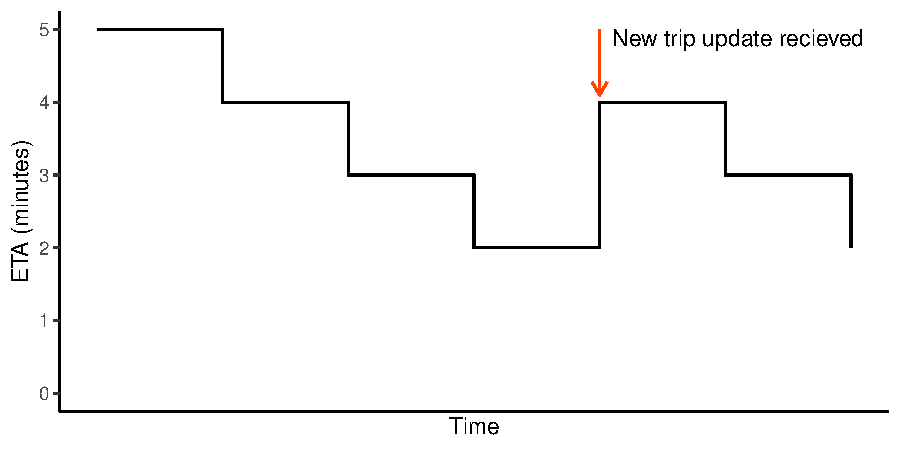
\includegraphics[width=.8\textwidth]{figure/tu_eta_jump-1} 

}

\caption[ETAs as percieved by passengers under the current system]{The current system displays \glspl{eta} to passengers as integer minutes which decrease over time. When new data is recieved (marked by an arrow) the \gls{eta} is updated, which may result in a sudden ``jump'', as demonstrated.}\label{fig:tu_eta_jump}
\end{figure}


\end{knitrout}


The reverse can also occur, for example, if for some reason the bus reports its arrival or departure late. However, more prevalent is that the update is skipped altogether, so a bus that was five minutes behind schedule has made up several minutes and arrives at the bus stop while the \gls{dms} still shows it as being two minutes away. At first, this may seem like a good thing: passengers at the stop have a shorter wait. Other passengers making their timely way to the bus, however, may have to sprint or miss the bus altogether, which is not ideal.


The main repercussion of the described issues is that arrival and departure time data become very noisy and difficult to trust. They do, however, provide a lot of information without which it would be challenging to infer the trajectory of a bus between stops---which is the primary aim of this part of our work. We discuss this further in \cref{sec:pf-likelihood} when we present the likelihood function.
